
\section*{Exercise 1}

Using 1000 randomly selected subperiods of 500 days, we need to show the instability of the weights of the optimal portfolio when we
\begin{enumerate}
\item update $\mu$ and $\Sigma$, meaning that we only use the subsample of 500 days instead of the entire sample of approximately 2000 days to calculate expected log-returns and volatility; 
\item update $\mu$ only, and we use the covariance matrix for the entire sample;
\item update $\Sigma$ only.
\end{enumerate}

Figure \ref{fig1} demonstrates the instability of the weights for the first 20 stocks of our dataset. We limited our boxplots to the first 20 stocks in order to give the reader a clearer view of the results, it has to be stressed that our calculations are not limited to 20 stocks but they include all the stocks composing the S\&P500. 
What we learned while doing this exercise is the importance of the number of days of observations we need in order to have a stable (here meaning invertible) covariance matrix that allows us to solve the Markowitz algorithm without excessively amplifying the magnitude of the optimal weights. An efficient and time-saving method to calculate the covariance matrix while using a computer is to use eigenvalues and eigenvectors to apply the spectral decomposition theorem. Applying the spectral theorem means building two matrices:
\begin{itemize}
\item	The first one is a diagonal matrix with eigenvalues on the diagonal and zeros elsewhere
\item The second one is built combining eigenvectors by column
\end{itemize}
Notice that the inverse of a diagonal matrix with the same allure of the first one just described is the same matrix but with coefficients on the diagonal in the form of $1/c_{ij}$ where $c_{ij}$ denotes the coefficients of the original matrix. When $c_{ij}$ are close to zero $1/c_{ij}$  tends to infinity and the correctness/stability of any linear transformation resulting from this matrix collapses.
When too few observations are used to calculate the covariance matrix, the risk of having very small coefficient on the diagonal grows. The unwanted result reflected on weights instability while applying the Markowitz optimization.
In the first series of graphs we are interested in determining whether the optimal weights variability is due to the sensibility of the estimate of mu or sigma.
In the first boxplot we determine the optimal weights using both mu and sigma estimates of the same subsample.
In the second boxplot we determine the optimal weights using the estimate of mu of the same subsample and the estimate of sigma of the entire sample.
In the third boxplot we determine the optimal weights using the estimate of sigma of the same subsample and the estimate of sigma of the entire sample.
As a result we see that weights instability and variability is primarily due to the estimation of sigma.


\begin{figure}[H]
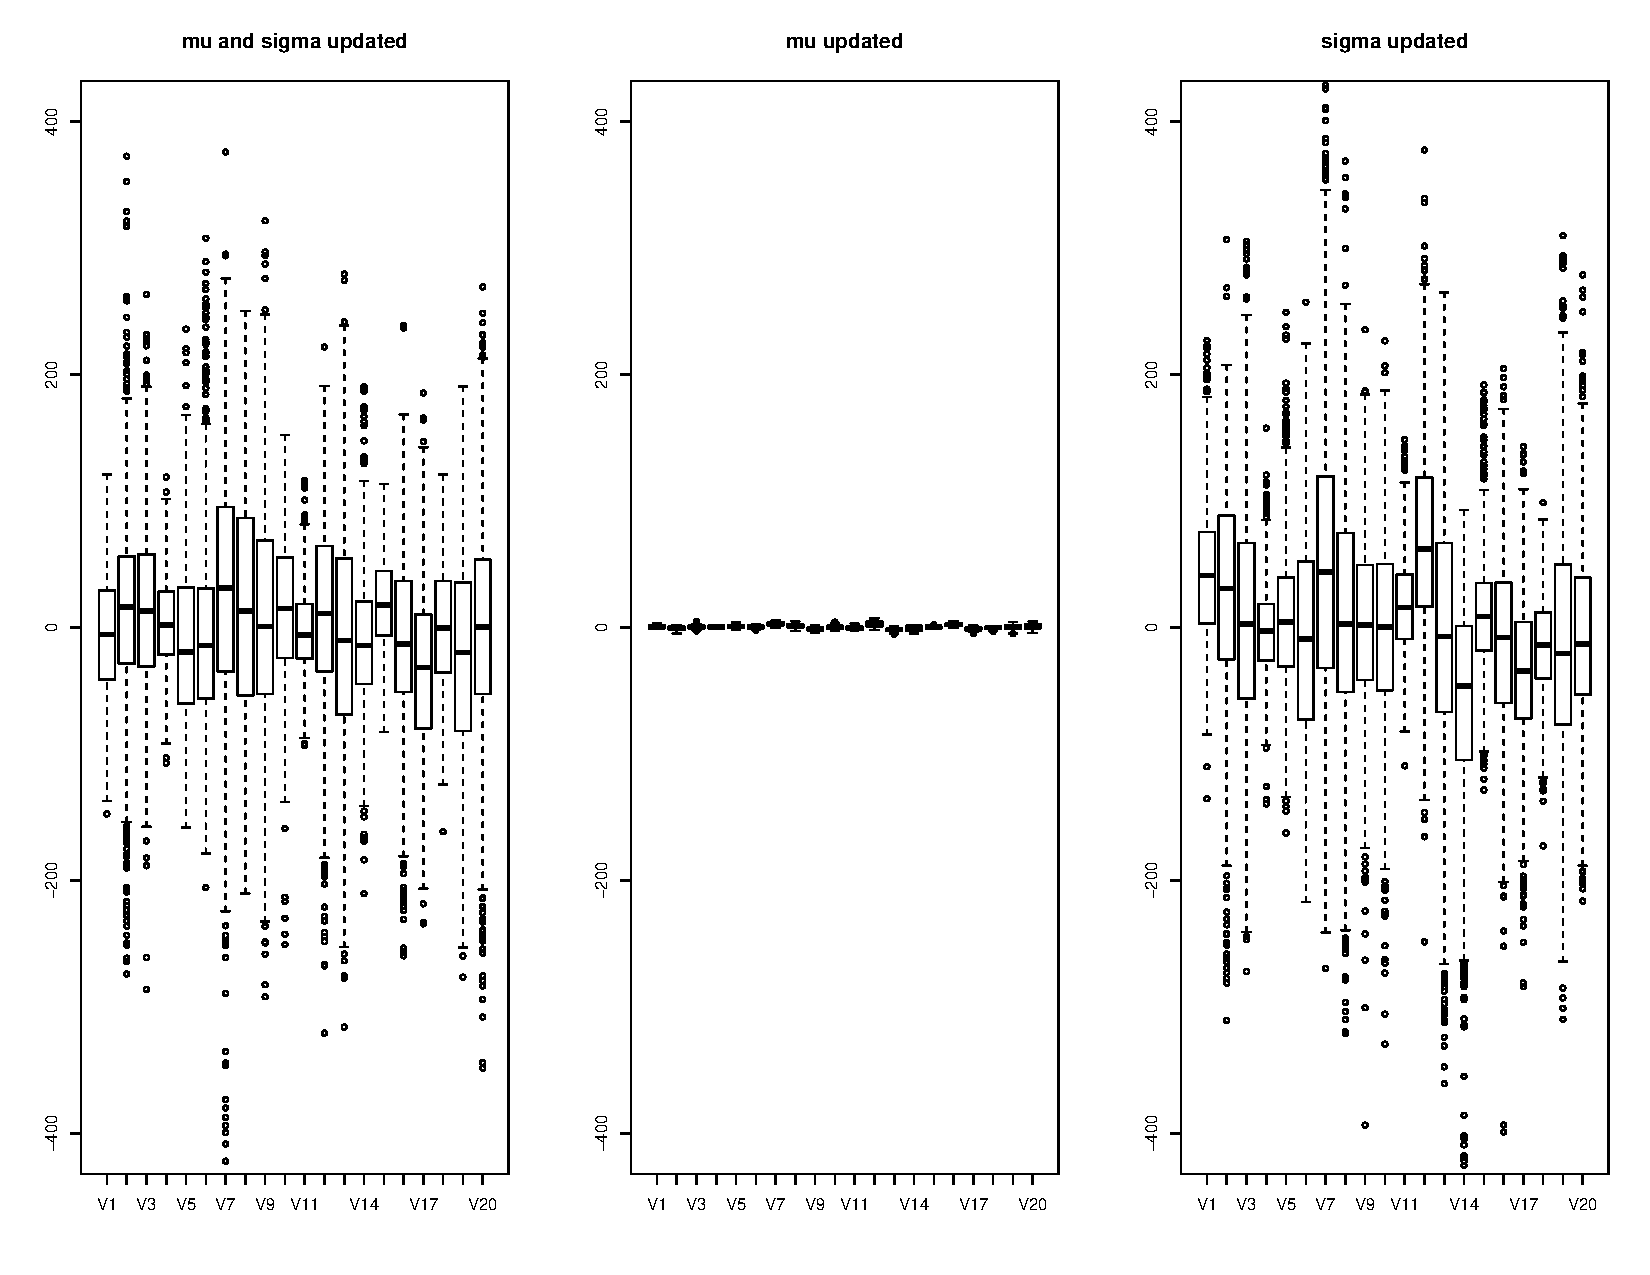
\includegraphics[width=15cm]{Boxplot_question_1.pdf}
\caption{Weight stability for a subsample of 500 days}
\label{fig1}
\end{figure}


We have used the following R code to generate boxplots: 
\begin{verbatim}

X=read.delim("data_lausanne_equity.csv",sep=";",header=FALSE)
X=diff(as.matrix(log(X)),1)

#Markowitz
mu=apply(X,2,mean)
sigma=cov(X)
sigmainv=solve(sigma)
gamma=3
w=1/gamma*sigmainv%*%mu

#subsampling
wtotal=c()            		#creates a vector to store the weights
wsigma=c()
wmu=c()
count=0                 		#counter defined and set to 0
for (i in 1:1000)        		#starts a 1000 rounds loop
{
 #generates a random number/date from the dataset matrix X 
  u=round(runif(1,500,nrow(X)),0)               	
  
  #creates a vector sample of 500 dates ending at day u					
  sample=X[(u-499):(u),]           
  
  #tests if sigma inverse can be calculated            		
  check=try(solve(var(sample)),silent=TRUE) 
 
  #if sigma is not invertible (try failed)   
  if (is.character(check))                     			
    {
      count=count+1            
    } else                                      			
    { 
      #calculates the mean of the subsample
      mutemp=apply(sample,2,mean)     
   
      #calculates sigma inverse of the subsample
      sigmainvtemp=solve(cov(sample))    

      #computes Markowitz weights using the sigma of the subsample 
      #and the population mean
      temp=1/gamma*sigmainvtemp%*%mu        
      wsigma=rbind(wsigma,t(temp))         
      
      #computes Markowitz using subsample mean and sigma  	 
      temp=1/gamma*sigmainvtemp%*%mutemp        
      wtotal=rbind(wtotal,t(temp))     
      
      #computes Markowitz using the population sigma and the subsample mean      		 
      temp=1/gamma*sigmainv%*%mutemp            
      wmu=rbind(wmu,t(temp))                   		 
      }
}
#plotting the results
layout(matrix(1:3,1,3))
boxplot([wtotal,1:20], main="mu and sigma updated", ylim=c(-400,400))
boxplot(wmu[,1:20], main="mu updated", ylim=c(-400,400))
boxplot(wsigma[,1:20], main="sigma updated", ylim=c(-400,400))

\end{verbatim}
\newpage
